\chapter{Unit 1B}

\section{Fictitious Forces and Apparent Weight}
\subsection{Fictitious Forces}
\red{Fictitious forces} are also called \red{apparent forces} or \red{perceived forces}

\begin{redblock}
    \textbf{Explanation:} When the object is viewed from a \red{non-intertial F.O.R, we created fictitious force to explain the motion and behavior}
\end{redblock}

The \red{fictitious forces} will always act in the direction opposite to the direction of acceleration of 
the frame of reference.\\

\begin{cyanblock}
    The magnitude of each fictitious force can be calculated by:
    \[
        F_{fict} = m|\vec{a_{F.O.R}}|
    \]
\end{cyanblock}

Perceived acceleration could be represented by \red{$\vec{a_{per}}$}

\begin{redblock}
    \textbf{Note: } The object's actual acceleration would be measured relative to an inertia FOR
\end{redblock}

\subsection{Apparent Weight}
Technically, this would be the sum of the \red{normal force} and the force of \red{friction} that a surface exerts 
on an object. 

\subsection{Some of the formulas}
\[
    \sum \vec{F} = m\vec{a_{per}}
\]

\section{Lecture 2.5}
\subsection{Uniform Circular Motion}
\begin{redblock}
    \textbf{Direction}: The velocity of an object at any point along a circle has a direction that is 
    \red{tangential} to the circle
\end{redblock}

\columnratio{0.6, 0.4}
\begin{paracol}{2}
    \begin{leftcolumn}
        \textbf{Question:} If an object is attached to a string, swung in a circular motion and then the string is released,
        which of the five paths shown here will the object take?\\
        \red{ANS: Path 2}
    \end{leftcolumn}

    \begin{rightcolumn}
        \begin{center}
            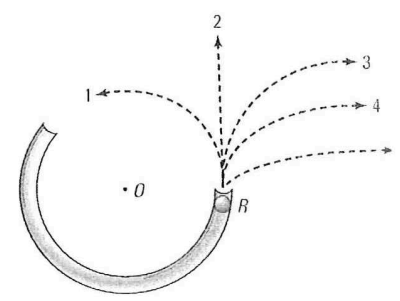
\includegraphics[width=0.3\textwidth]{graph/circularMotion.png}
        \end{center}
    \end{rightcolumn}
\end{paracol}

\subsection{Centripetal acceleration}
From the \red{Newton second law}, we understand that \red{An object will accelerate in the same 
direction as the net force}.

If the centripetal force is directed toward the centre of the circle, then what direction is the acceleration in?
\red{ANS: Toward the circle}

In other words, the acceleration will always \red{perpendicular} to the velocity of the object.

\subsection{Formulas}
\begin{cyanblock}
    Formula 1:
    \[
        \vec{a_{c}} = \frac{4 \pi ^2 R}{T^2}
    \]
    \[
        \vec{a_{c}} = 4\pi ^2 R f^2
    \]
    \[
        \vec{a_{c}} = \frac{V^2}{R}
    \]
    \begin{center}
        $\vec{a_{c}}$ is the acceleration of the object in $\frac{m}{s^2}$\\
        $R$ is the radius of the circular path that the object is moving around (in $m$)\\
        $T$ is the period of the object's motion \\
        $v$ is the speed of the object in (m/s)
    \end{center}
\end{cyanblock}

\begin{cyanblock}
    For clockwise:
    \begin{center}
        direction of acceleration = direction of velocity + 90 degree
    \end{center}
    else:
    \begin{center}
         direction of acceleration = direction of velocity - 90 degree
    \end{center}
\end{cyanblock}

\section{Motion of a car on Banked Turn}
\begin{center}
    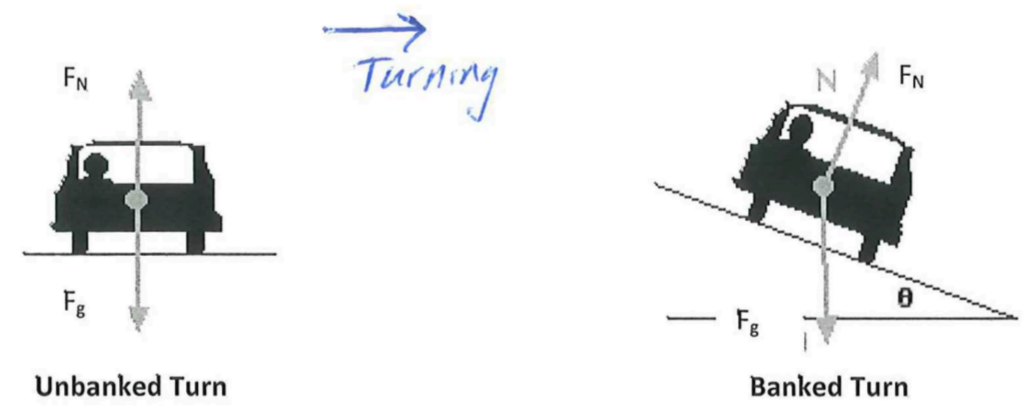
\includegraphics[width=0.7\textwidth]{graph/BankedTurn.png}
\end{center}
\subsection{Forces}
For \red{unbanked Turn}, \red{Static friction} contribute to the centripetal force

For \red{Banked Turn}, both \red{static friction} and \red{normal force} contribute to the centripetal force

\subsection{Critical Speed}
\begin{definition}
    Critical speed the minimum speed needed at which a vehicle can travel around a curve, baked road without relying on static friction
\end{definition}

The formula for critical speed is defined as:
\begin{cyanblock}
    \[
        v = \sqrt{R*tan\theta *g}
    \]
    \begin{center}
        $v$ = Critical Speed\\
        $R$ = The radius of the banked turn\\
        $g$ = The acceleration by Gravity\\
    \end{center}
\end{cyanblock}

Above the \red{critical speed}, the car wants to go \blue{up}. At this case, friction must act \red{down the bank} to prevent sliding outward

Below the \red{critical speed}, the car wants to go \blue{down}. At this case, friction must act \red{up the bank} to prevent sliding inward

\section{Universal Gravitation, Gravitational field}
\subsection{Force of Gravity}
The formula for the \textbf{Force of Gravity} acting between two objects is:
\[
    Fg = \frac{G * m_{1} * m_{2}}{R^2}
\]
\begin{center}
    $Fg$ = the magnitude of the force of gravity that $m_{1}$ exerts on $m_{2}$ and $m_{2}$ exerts on $m_{1}$\\
    $G$ = Universal Gravitational Constant\\
    $m_{1}$ = the mass of one of the objects (in kg)\\
    $m_{2}$ = the mass of the other object (in kg)\\
    $R$ is the distance separating the objects' \red{center of mass} in (m)
\end{center}

\red{Remainder:} \textbf{Altitude} refers to the distance between the Earth's surface and the object!\\

In reality, \red{every particle} in A exerts a force of gravity on every particle in B. 
If the objects (A and B) are relatively close together and large (relative to their separation distance)
then these forces are not parallel.
\begin{center}
    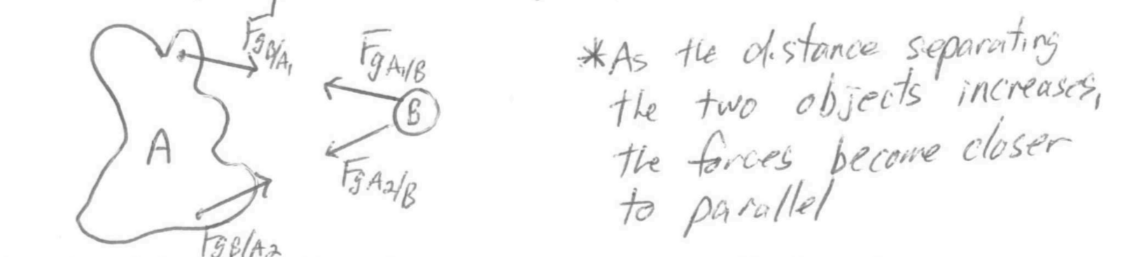
\includegraphics[width=0.8\textwidth]{graph/fgparallel.png}
\end{center}

The \textbf{formula works} best for two objects who \red{seperation distance} is \red{very large} relative to their sizes, 
or when both object are perfect \red{sphere}\\

The \textbf{formula works well} for a very, very \red{large} sphere (whose mass is uniformly distributed through out)
and a relatively \red{small} object on its surface\\

You can not use this formula when one object is \red{inside} of another object!

\subsection{Gravational Fields}
\begin{definition}
    \textbf{A force field} is a region surrounding an object in which the object is capable of exerting a force on another object
\end{definition}

A \red{Gravational field} is a region surrounding an object in which the object is capable of exerting a force of gravity 
on another object.

\subsection{Differences between strength of gravity and acceleration}
Acceleration due to gravity:
\begin{center}
    Units: \blue{$\frac{m}{s^2}$}\\
    What does it imply?:  \blue{When an object is in free fall, it will accelerate at that rate}\\
    When is it true: \blue{Only when $Fg$ is the only force on the object}
\end{center}

Gravitational field strength:
\begin{center}
    Units: \blue{$\frac{N}{kg}$}\\
    What does it imply?:  \blue{When an object is in free fall, it will accelerate at that rate}\\
    When is it true: \blue{Gravity is exertings a force of $\mid \vec{g} \mid $ Newtons for each Kg of mass}
\end{center}

Specific types of field strengths are \red{additive}. The \red{net gravitational field strength} at a location is the \red{sum}
of all the individual strengths of gravitational fields at that location OR $\sum \vec{g} = \vec{g_{1}} + \vec{g_{2}}$\\

When you need to calculate \blue{magnitude} of Gravational field from that object $M$ exerts on $m$:
\begin{equation} \label{eq:1}
    Fg_{M/m} = \frac{GMm}{R^2}
\end{equation}
\begin{equation} \label{eq:2}
    Fg_{M/m} = mg
\end{equation}
Add \ref{eq:1} and \ref{eq:2}
\begin{equation}
    g = \frac{GM}{R^2}
\end{equation}
\begin{center}
    $g$ is the \blue{magnitude of the grav field strength} of $M$, at a specific location (in $N/kg$)\\
    $R$ is the distance that the location is from $M$'s centre of mass(in m)\\
    $G$ is the universal gravitational constant ($G$ = $6.67*10^{-11}\frac{Nm^2}{Kg^2}$)
\end{center}

\section{Satellites}
A satellite is an object that \red{orbits around another object}\\

There are \textbf{natural} satellites and \textbf{artifical} object
\begin{itemize}
    \item The moon is a \textbf{natural} satellite of the Earth
    \item The international space station (ISS) is an \textbf{artifical} object
\end{itemize}

\subsection{Netwon's Cannon}
His idea was: \textit{if a cannon is placed on the top of a very tall mountain, and if you could ignore air resistance. The cannon 
shoots a cannonball horizontal}\\

At the idea speed: the distance the cannonball has fall \textbf{equals} the distance that the Earth has \textbf{turned away}\\

If $v  < v_{idea}$, the distance between the ball and Earth's surface will \textbf{decrease}\\

If $v  > v_{idea}$, the distance between the ball and Earth's surface will \textbf{increase}\\

The cannon must has a constant speed and travel in the perfect circular path

\subsection{Geosynchronous}
They have the same orbital period as the \textbf{rotational speed} of the object they are on the ground\\

The period is around \textbf{24 hrs}\\

There is a special type of geosynchronous is called \textbf{Geostationary}
\begin{itemize}
    \item "Hang above" a location on Earth's \textbf{Equator}
    \item They orbit in the same \textbf{direction} that the Earth rotates
\end{itemize}

\subsection{Formulas related to satellite}
\begin{equation}
    v = \sqrt{\frac{GM}{R}}
\end{equation}
\begin{equation}
    T = \sqrt{\frac{4 \pi^2 R^3}{GM}}
\end{equation}
\begin{center}
    $v$ is the velocity of the satellite\\
    $T$ is the period of the satellite
\end{center}

Next section is the last section of this unit!

\section{Rotating Frame of Reference}
\subsection{Little problem}
When a person is standing (on Earth) there are two forces acting on them:\\

\columnratio{0.4, 0.6}
\begin{paracol}{2}
    \begin{leftcolumn}
        \begin{figure} \label{fig:2.1}
        \centering
            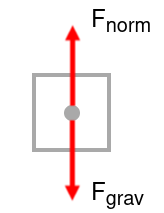
\includegraphics[width=0.2\textwidth]{graph/FBD2.6.1.png}
        \caption{Normal force and Gravity}
        \end{figure}
        
    \end{leftcolumn}

    \begin{rightcolumn}
        The normal force acting on the person is pushing force, thus a force of \textbf{compresion}. An object 
        that has a compression force must be able to \textbf{withstand this force} or it will collapse. (See \ref{fig:2.1})\\

        In the caes of a person, their muscles and their bones must be able to withstand this force, thus you 
        \textbf{muskule-skeletal system develops} to withstand this force
    \end{rightcolumn}
\end{paracol}

When a person is in orbit around a planet, there is only the force of gravity acting on them! They are in 
\textbf{constant state of free fall} 

